\documentclass{classrep}
\usepackage[utf8]{inputenc}
\frenchspacing

\usepackage{graphicx}
\usepackage[usenames,dvipsnames]{color}
\usepackage[hidelinks]{hyperref}
\usepackage{lmodern}
\usepackage{graphicx}
\usepackage{placeins}
\usepackage{url}
\usepackage{amsmath, amssymb, mathtools}
\usepackage{listings}
\usepackage{fancyhdr, lastpage}

\pagestyle{fancyplain}
\fancyhf{}
\renewcommand{\headrulewidth}{0pt}
\cfoot{\thepage\ / \pageref*{LastPage}}

%--------------------------------------------------------------------------------------%
\studycycle{Informatyka stosowana, studia dzienne, II st.}
\coursesemester{I}

\coursename{Wprowadzenie do Data Science i metod uczenia maszynowego}
\courseyear{2020/2021}

\courseteacher{mgr inż. Rafał Woźniak}
\coursegroup{Wtorek, 13:15}

\author{%
    \studentinfo[239661@edu.p.lodz.pl]{Szymon Gruda}{239661}
}

\title{Zadanie 1.: Problem Set 1}

\begin{document}
    \maketitle
    \thispagestyle{fancyplain}

    \section{Wprowadzenie} {
        Dane wraz ze wykorzystującą je statystyką pozwalają opisywać otaczający ludzi świat i informować co się w nim dzieje.
         Bardzo ważnym aspektem jest ich prezentacja (wizualizacja). Dużo trudniej jest ludziom zinterpretować długą tabelę 
         z samymi liczbami, lepszą metodą jest zwizualizowanie danych, np. poprzez wykres. Niestety wizualizowanie danych
          jest podatne na różnego rodzaju manipulacje, które zostaną omówione poniżej.
    }

    \section{Przykłady manipulacji danymi podczas ich wizualizacji} {
        % \begin{figure}[hbt!]
              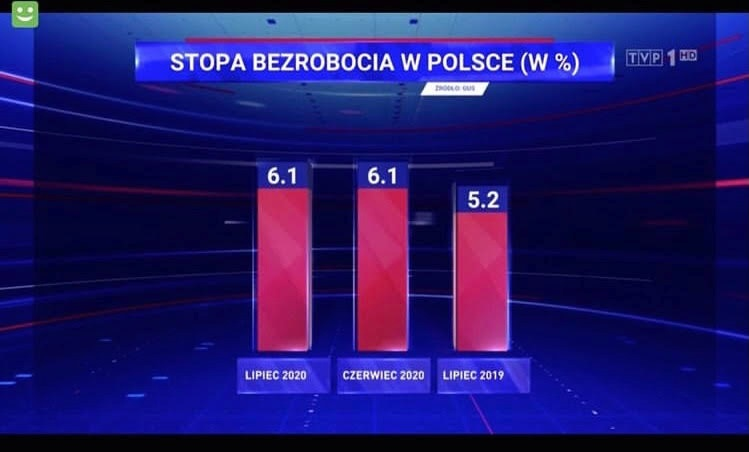
\includegraphics[width=\linewidth]{1.jpg}
              \caption{tvp xd}
              \label{fig:rysunek1}
        % \end{figure}
       \par
       Rysunek \ref{fig:rysunek1} przedstawia wykres stopy bezrobocia w Polsce.
       Wykres na pierwszy rzut oka wskazuje, że stopa bezrobocia maleje. Niestety tak nie jest, okazuje się że autor wykresu,
        miesiąc chronologicznie późniejszy umieścił wcześniej. Dodatkowo dziedzina danych to bardzo wąski zbiór trzech miesięcy,
         przez co wykres nie obrazuje sytuacji w ciągu całego jednego roku, dopuszczalne byłoby przedstawienie danych zebranych
          w ramach jednego kwartału, ale nie trzech różnych miesięcy, na przestrzeni dwóch lat.
       
        % \begin{figure}[hbt!]
              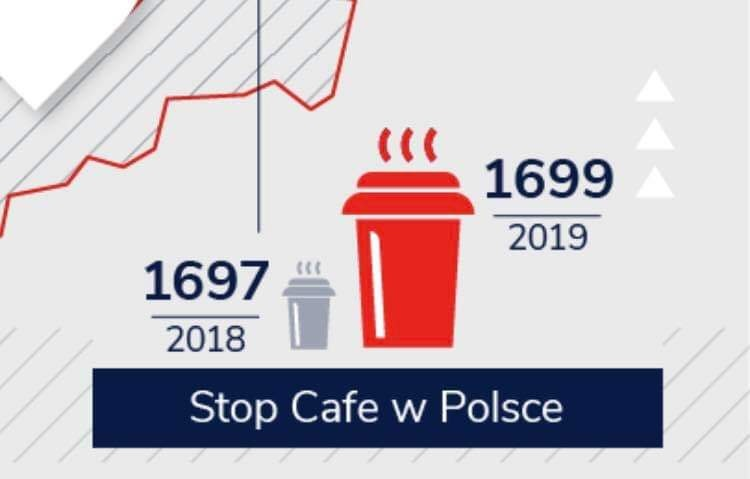
\includegraphics[width=\linewidth]{2.jpg}
              \caption{h,,,}
              \label{fig:rysunek2}
        % \end{figure}
        \par
       Rysunek \ref{fig:rysunek2} przedstawia "dynamniczny wzrost liczby stop cafe w Polsce". Infografika nie zawiera dokładnej 
       informacji co prezentuje, ale można się domyślać że liczbę kawiarni na przestrzeni dwóch lat. 
       Liczby zostały przedstawione jako dwa kubki kawki, jeden jest dwukrotnie mniejszy od drugiego.
        Czytelnik mógłby wywnioskować na podstawie samej grafiki, że ma doczynienia z dwukrotnym wzrostem liczby, 
        otóż nie, podane obok kubków liczby prezentują wzrost liczby kawiarni o 2.
       
}

    
    \section{Wnioski} {
        Podsumowując wykonane zadanie wnioskuje, że:
        \begin{itemize}
            \item ...

        \end{itemize}
    }

    \begin{thebibliography}{0}
        \bibitem{l2short}{ }
        \bibitem{l2short}{ }
    \end{thebibliography}

\end{document}
